\hypertarget{Project Management}{%
\section{Project Management}\label{Project Management}}

\hypertarget{Materials and Methods}{%
\subsection{Materials and Methods}\label{Materials and Methods}}

Following is a brief summary of the tools (Fig. \ref{fig: figure1}) that went into designing and implementing this project:

\begin{itemize}
    \item \textbf{Digital Twin Ecosystem:} \href{https://autodrive-ecosystem.github.io}{AutoDRIVE Ecosystem}
    \item \textbf{Vehicle Platforms:} \href{https://youtu.be/YFQzyfXV6Rw?feature=shared}{Nigel}, \href{https://youtu.be/Rq7Wwcwn1uk?si=_ODExkHBopsQszrU}{F1TENTH}, \href{https://global.agilex.ai/chassis/9}{Hunter SE} and \href{https://youtu.be/YIZz_8rLgZQ?si=6Z6LWxWSTyS3Uk8u}{OpenCAV}
    \item \textbf{Software Stack:} \href{https://github.com/autowarefoundation/autoware.universe/tree/galactic}{Autoware Universe - ROS 2 Galactic}
    \item \textbf{Programming:} \href{https://www.python.org}{Python} and \href{https://isocpp.org}{C++}
\end{itemize}

\begin{figure}[htpb]
    \centering
    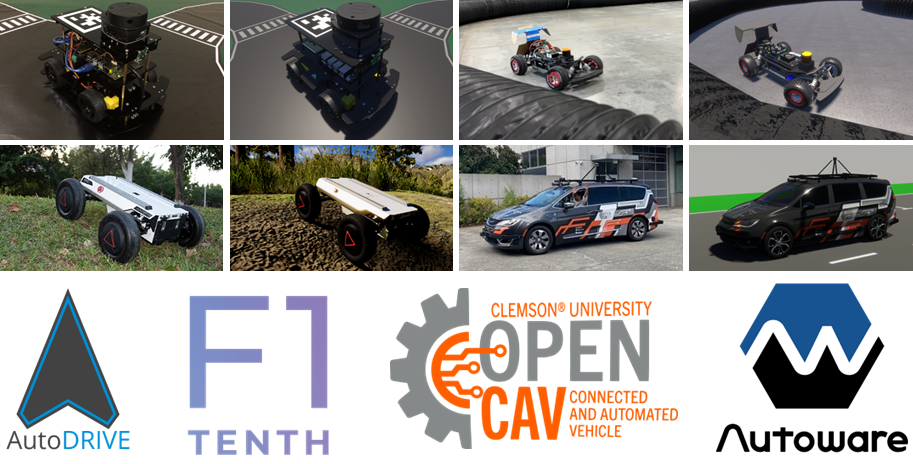
\includegraphics[width=\linewidth]{Figures/fig2.png}
    \caption{Project tools: AutoDRIVE Ecosystem employed to develop autonomy-oriented digital twins of small-scale (Nigel and F1TENTH), mid-scale (Hunter SE) and full-scale (OpenCAV) vehicles for deploying the Autoware stack.}
    \label{fig: figure2}
\end{figure}

The vehicles used for this project varied across scales (Fig. \ref{fig: figure2}). Small-scale platforms included Nigel (1:14 scale) and F1TENTH (1:10 scale), mid-scale platforms included Hunter SE (1:5 scale) and full-scale platforms included the OpenCAV (1:1 scale). Consequently, the sensor suite for Nigel and F1TENTH\footnote{The virtual F1TENTH was modeled with all sensors modules but only a subset of them were used for physical deployments} included small-scale sensors such as throttle and steering sensors, incremental encoders, indoor-positioning system (IPS), inertial measurement unit (IMU), RGB cameras and a 2D LIDAR. Alternatively, the sensor suite for Hunter SE and OpenCAV included different variants of 3D LIDARs in addition to similar virtual sensors. The actuators for small and mid-scale vehicles comprised throttle and steering actuators, which provided driving and steering torques to the respective wheels. Alternatively, the OpenCAV had a detailed powertrain model and exhaustive control inputs (throttle, steering, brake, handbrake) corresponding to its real-world counterpart. Finally, each vehicle was simulated in environment(s) appropriate for its scale and operational design domain.

For digital twinning, we adopted \href{https://github.com/Tinker-Twins/AutoDRIVE/tree/AutoDRIVE-Simulator}{AutoDRIVE Simulator}, a high-fidelity simulation system for autonomy-oriented applications. The simulation models were calibrated and benchmarked against their real-world counterparts for perception and dynamics reliability. The same simulation framework was also used to develop various HMIs that could directly interface with the virtual vehicles.

Core API development along with Autoware integration for all the virtual/real vehicles was accomplished using \href{https://github.com/Tinker-Twins/AutoDRIVE/tree/AutoDRIVE-Devkit}{AutoDRIVE Devkit}. The developed APIs could interface the virtual/real vehicles with Python, C++, ROS \cite{ROS1}, ROS 2 \cite{ROS2} or the Autoware stack. Additionally, the said framework also facilitated the development of API-mediated HMIs for the virtual as well as physical vehicles. 

Finally, we employed \href{https://github.com/Tinker-Twins/AutoDRIVE/tree/AutoDRIVE-Testbed}{AutoDRIVE Testbed} for sim2real deployment of Autoware demonstrations, which was integrated with \href{https://github.com/Tinker-Twins/AutoDRIVE/tree/AutoDRIVE-Devkit}{AutoDRIVE Devkit} deployed on Nigel and F1TENTH.

\hypertarget{Work Breakdown Structure}{%
\subsection{Work Breakdown Structure}\label{Work Breakdown Structure}}

For our convenience, we divided the project into 3 phases, each focusing on a different scale of autonomous vehicle platform for developing vehicle and environment digital twins, integrating various APIs and HMIs, and demonstrating an end-to-end autonomy deployment using the Autoware stack. The first phase of the project was set as the core deliverable and the rest of them as ``ambitious'' extensions subject to time-availability:
\begin{itemize}
    \item \textbf{Phase 1: Small-Scale Deployments:}
    \begin{itemize}
    \item Develop digital twins of Nigel and F1TENTH vehicles
    \item Develop digital twins of small-scale environments suitable for respective vehicles
    \item Develop APIs and HMIs to connect with virtual and real vehicles
    \item Integrate Autoware stack with virtual and real vehicles
    \item Demonstrate sim2real deployment of Autoware stack on both the vehicles
    \end{itemize}

    \item \textbf{Phase 2: Mid-Scale Deployments:}
    \begin{itemize}
    \item Develop digital twins of Hunter SE and Husky robots
    \item Develop digital twins of mid-scale environments suitable for respective vehicles
    \item Develop APIs and HMIs to connect with virtual and real vehicles
    \item Integrate Autoware stack with virtual and real Hunter SE
    \item Demonstrate simulated deployment of Autoware stack on Hunter SE
    \end{itemize}

    \item \textbf{Phase 3: Full-Scale Deployments:}
    \begin{itemize}
    \item Develop digital twins of OpenCAV and RZR vehicles
    \item Develop digital twins of full-scale environments suitable for respective vehicles
    \item Develop APIs and HMIs to connect with virtual and real vehicles
    \item Integrate Autoware stack with virtual and real OpenCAV
    \item Demonstrate simulated deployment of Autoware stack on OpenCAV
    \end{itemize}
\end{itemize}

\hypertarget{Project Timeline}{%
\subsection{Project Timeline}\label{Project Timeline}}

As mentioned earlier, we split this project into three phases viz. small-scale, mid-scale and full-scale Autoware deployments. Additionally, logistical tasks such as continuous documentation, preparation of slide decks, presentation rehearsals, report writing, etc. had to be accounted for in the overall project plan and strictly followed to ensure successful completion of the project.

\begin{figure}[htpb]
    \centering
    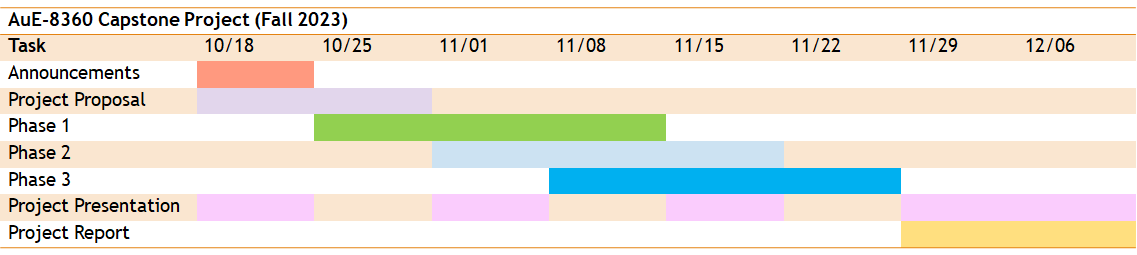
\includegraphics[width=\linewidth]{Figures/fig3.png}
    \caption{Project timeline Gantt chart.}
    \label{fig: figure3}
\end{figure}

Given the overall timeline from 10/18/2023 to 12/13/2023 (end of Fall 2023 semester), the milestones and deliverables of the project were planned as indicated in (Fig. \ref{fig: figure3}), which depicts the Gantt chart. It is to be noted that factors such as known parallel commitments were weighed in while preparing the timeline to enable practical adherence.


\hypertarget{Responsibility Assignment}{%
\subsection{Responsibility Assignment}\label{Responsibility Assignment}}

We divided the project into a set of tasks and assigned a subset of the team members with a primary and secondary responsibility of accomplishing each task as per the planned deadlines. Upon successful implementation of the project, albeit barebone, we came together for overall project optimization, organization and documentation.

\begin{itemize}
    \item \textbf{Primary responsibilities for Tanmay:}
    \begin{itemize}
    \item Develop digital twins of Hunter SE and Husky robots
    \item Develop digital twins of OpenCAV and RZR vehicles
    \item Develop digital twins of mid-scale environments suitable for respective vehicles
    \item Develop digital twins of full-scale environments suitable for respective vehicles
    \item Design and develop physical prototype of the Nigel (4WD4WS) vehicle
    \item Demonstrate sim/real deployment of Autoware stack on all the vehicles
    \end{itemize}
    
    \item \textbf{Primary responsibilities for Chinmay:}
    \begin{itemize}
    \item Develop digital twins of Nigel and F1TENTH vehicles
    \item Develop digital twins of small-scale environments suitable for respective vehicles
    \item Setup and calibrate physical prototype of the F1TENTH vehicle
    \item Develop APIs and HMIs to connect with virtual and real vehicles
    \item Integrate Autoware stack with virtual and real vehicles
    \item Project presentations, report and documentation
    \end{itemize}
\end{itemize}

It is to be noted that ``responsibility'' does not directly indicate ``contribution''. The team members have contributed equally and have no conflict of interest to declare.
